% HMC Math dept HW template example
% v0.04 by Eric J. Malm, 10 Mar 2005
\documentclass[12pt,letterpaper,boxed,cm]{hmcpset}

% set 1-inch margins in the document
\usepackage[margin=1in]{geometry}
\usepackage{mathtools}
\usepackage{mathrsfs}
% include this if you want to import graphics files with /includegraphics
\usepackage{graphicx}
\usepackage{cases}
\usepackage{hyperref}
\usepackage{siunitx}
\usepackage{tikz}
\usepackage{cases}
\usepackage{mathalfa}
\usetikzlibrary{arrows}

% info for header block in upper right hand corner
\name{Name: ~~~~~~~~~~~~~~~~~~~~~~~~~~~~~~~}
\class{Physics 51}
\assignment{Homework \#15}
\duedate{October 31, 2016}

\newcommand{\ev}[2]{\Big|_{#1}^{#2}}
\newcommand{\evv}[2]{\Big|_{#1}^{#2}}
\newcommand{\set}[1]{\left\{#1\right\}}
\newcommand{\s}[1]{\sqrt{#1}}
\newcommand{\f}[2]{\frac{#1}{#2}}
\newcommand{\p}[2]{\frac{\partial #1}{\partial #2}}
\providecommand{\t}[1]{\text{#1}}
\providecommand{\span}[1]{\text{span}\left(#1\right)}
\providecommand{\set}[1]{\left\{#1\right\}}
\providecommand{\l}[0]{\left}
\providecommand{\r}[0]{\right}
\newcommand{\m}[1]{\begin{matrix}#1\end{matrix}}
\newcommand{\bm}[1]{\begin{bmatrix}#1\end{bmatrix}}
\renewcommand{\bf}[1]{\mathbf{#1}}
\newcommand{\pn}[1]{\left( #1 \right)}
\newcommand{\abs}[1]{\left| #1 \right|}
\newcommand{\bk}[1]{\left[ #1 \right]}
\newcommand{\cis}[1]{\pn{\cos\pn{#1} + i\sin\pn{#1}}}
\newcommand{\cisi}[1]{\pn{\cos\pn{#1} - i\sin\pn{#1}}}
\renewcommand{\Im}[1]{\text{Im}\pn{#1}}
\renewcommand{\Re}[1]{\text{Re}\pn{#1}}
\renewcommand{\k}[0]{\f{1}{4\pi\epsilon_0}}
\renewcommand{\part}[1]{\vspace{1em}\noindent(#1)}

\makeatletter
\renewcommand*\env@matrix[1][*\c@MaxMatrixCols c]{%
  \hskip -\arraycolsep
  \let\@ifnextchar\new@ifnextchar
  \array{#1}}
\makeatother
\begin{document}
\problemlist{SUP1, SUP2, 38-P3, 34-P6*}

\begin{problem}[SUP1]
A parallel plate capacitor has circular plates of radius $R$ and separation $d$. The capacitor is connected to a battery of voltage $V$ and then disconnected so that the charge ought to remain constant. The air is humid, however, and therefore slightly conducting; thus the stored charge leaks back across the air gap between the capacitor plates at rate $i_\text{leak}$. Assume that this leakage current is uniformly distributed across the area of the plates. Find the magnetic field everywhere between the plates. 	
\end{problem}
\begin{solution}
\end{solution}
\newpage


\begin{problem}[SUP2]
In a material of non-zero electrical resistivity $\rho$, the relationship between electric field and current density is $\vec{E} = \rho\vec{j}$. For copper, $\rho = \SI{2e-8}{\ohm m}$. A copper wire with a circular cross-sectional area of \SI{4}{mm^2} carries a current of \SI{40}{A}.
\begin{enumerate}
	\item[(a)] What is the longitudinal electric field (field along the length of the wire) in the copper?
	\item[(b)] If the current is changing at a rate of \SI{5000}{A/s}, at what rate is $\vec{E}$ changing, and what is the resulting displacement current?
	\item[(c)] Does the displacement current contribute significantly to the magnetic field outside the wire? Explain your answer.	
\end{enumerate}
\end{problem}
\begin{solution}
\end{solution}
\newpage


\begin{problem}[38-P3]
The capacitor in Fig 38-25 consisting of two circular plates with radius $R = \SI{18.2}{cm}$ is connected to a source of emf $\mathscr{E} = \mathscr{E}_m\sin~\omega t$, where $\mathscr{E}_m = \SI{225}{V}$ and $\omega = \SI{128}{rad/s}$. The maximum value of the displacement current is $i_d = \SI{7.63}{\micro A}$. Neglect fringing of the electric field at the edges of the plates.
\begin{enumerate}
	\item[(a)] What is the maximum value of the current $i$?
	\item[(b)] What is the maximum value of $\f{d\Phi_E}{dt}$, where $\Phi_E$ is the electric flux through the region between the plates?
	\item[(c)] What is the separation $d$ between the plates?
	\item[(d)] Find the maximum value of the magnitude of $\vec{\mathbf{B}}$ between the plates at a distance $r = \SI{11.0}{cm}$ from the center.
\end{enumerate}
\begin{center}
	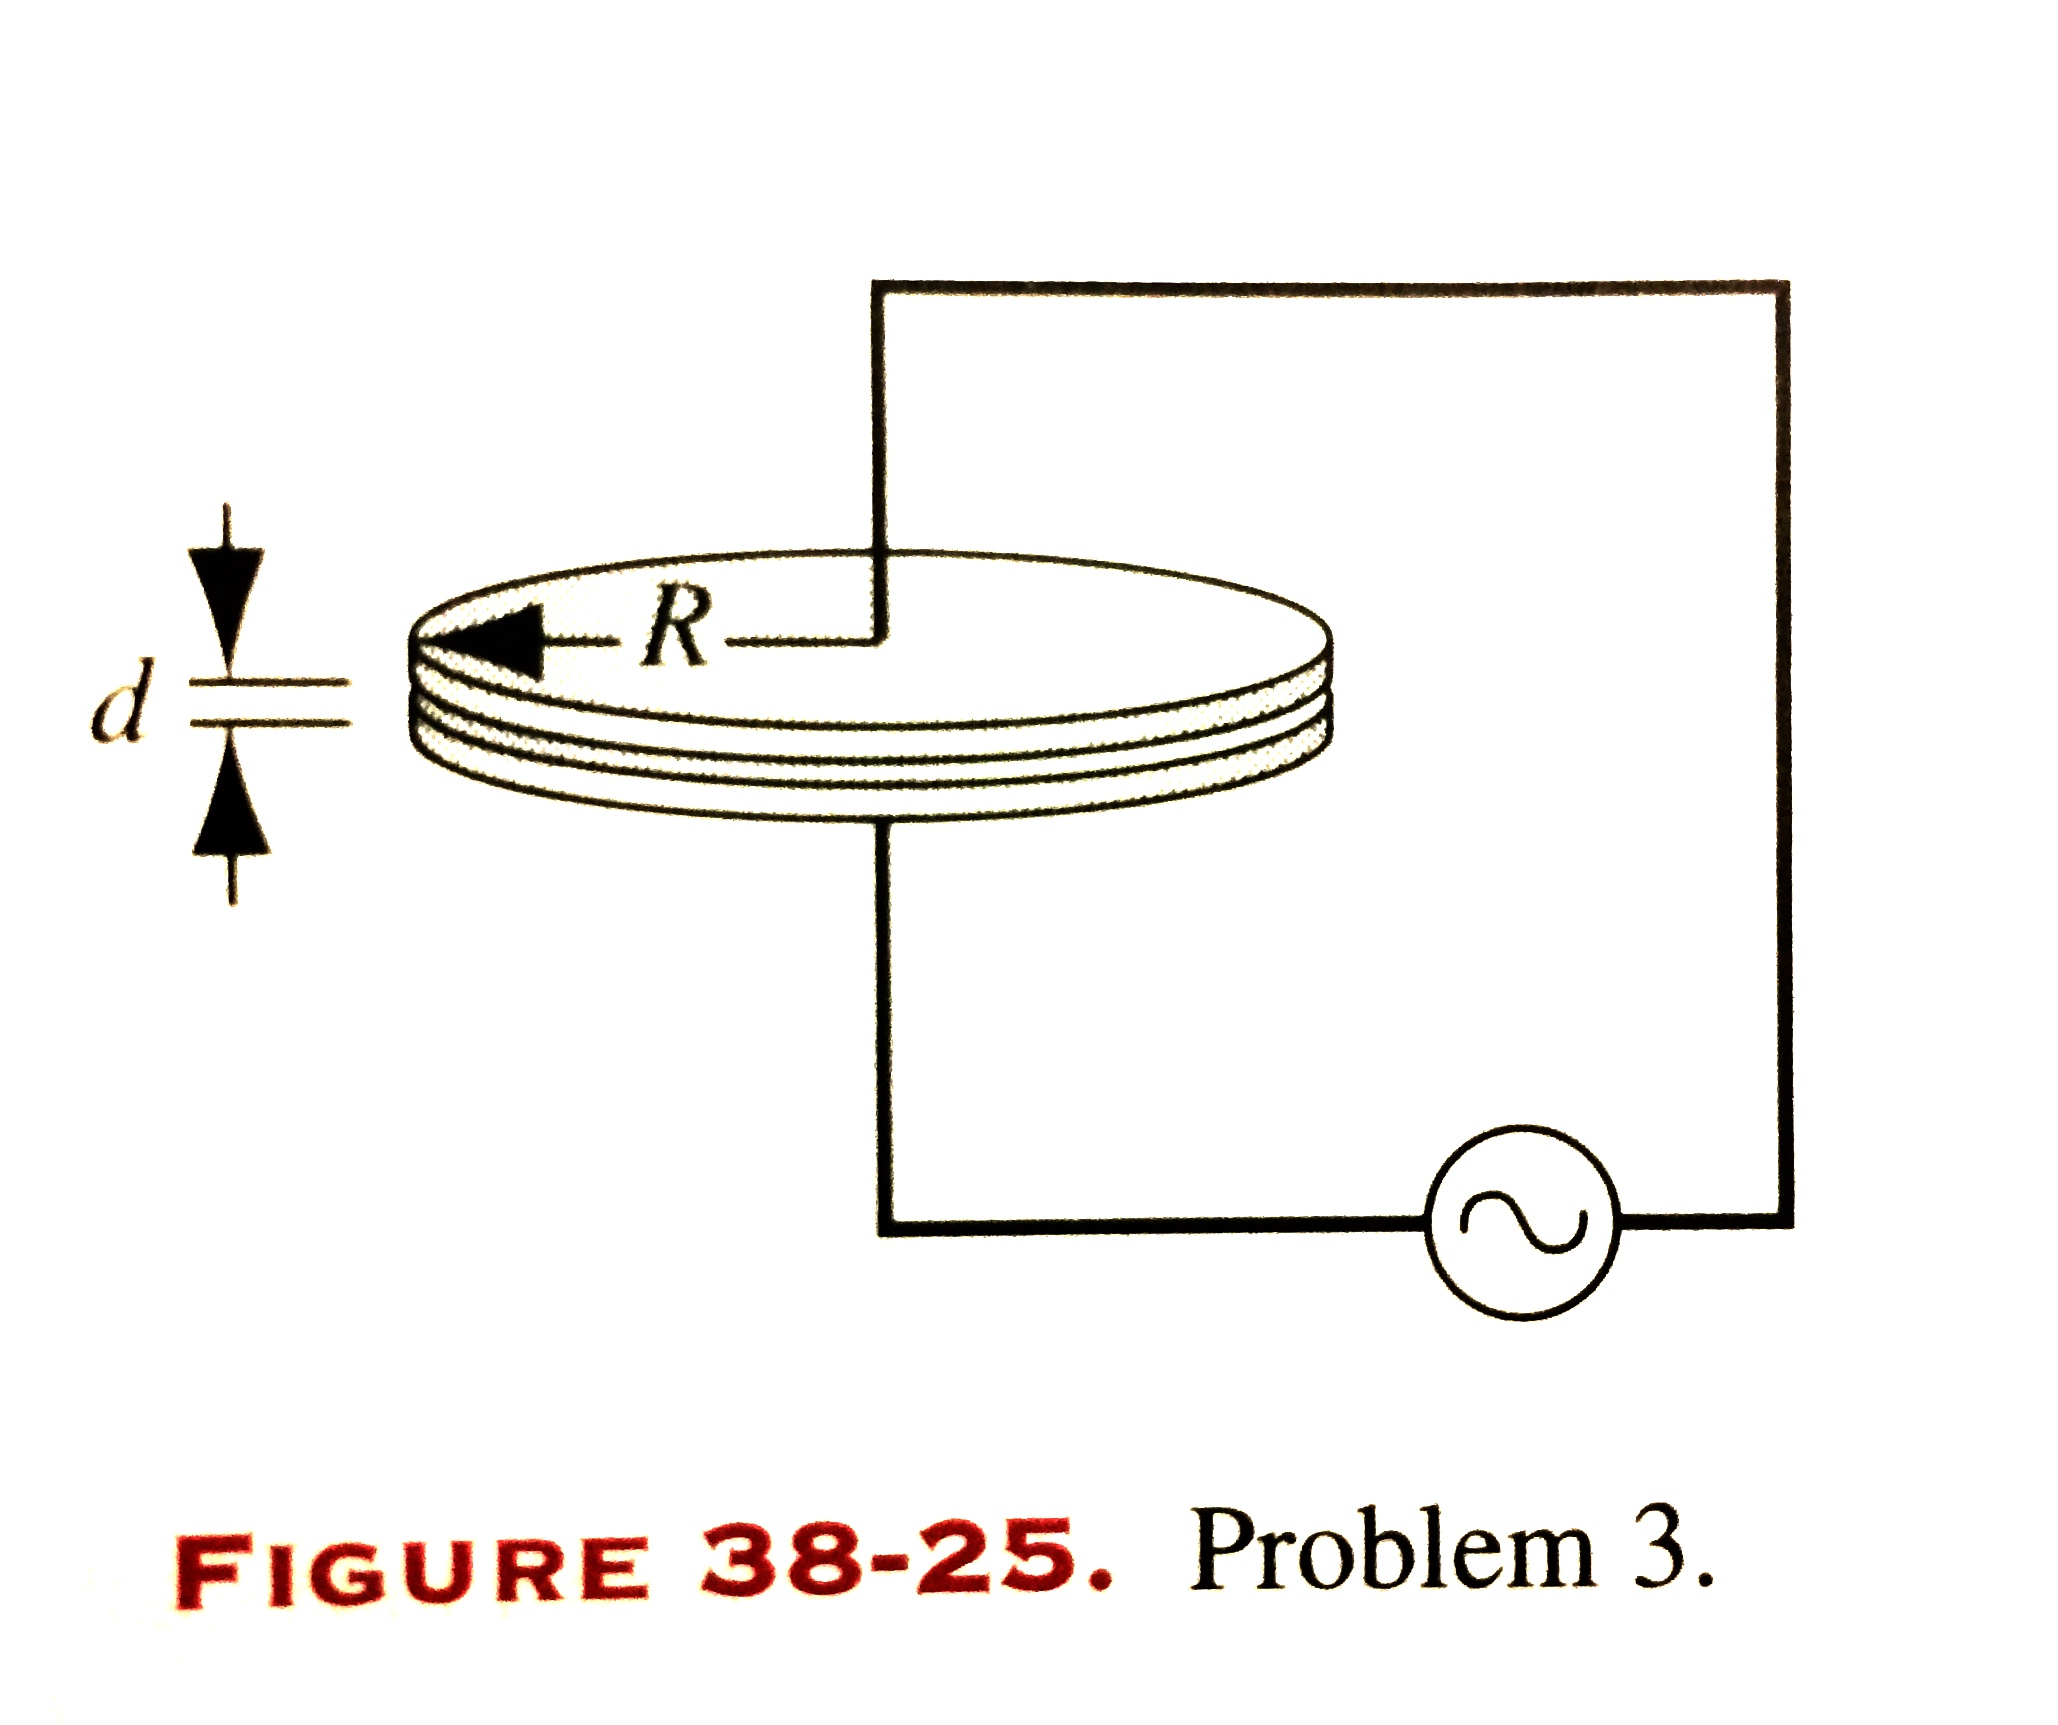
\includegraphics[scale=0.1]{01.jpg}
\end{center}
\end{problem}
\begin{solution}
\end{solution}
\newpage


\begin{problem}[34-P6*]
Figure 34-57 shows two parallel loops of wire having a common axis. The smaller loop (radius $r$) is above the larger loop (radius $R$), by a distance $x \gg R$. Consequently the magnetic field, due to the current $i$ in the larger loop, is nearly constant throughout the smaller loop and equal to the value of the axis. Suppose that $x$ is increasing at the constant rate $\f{dx}{dt} = v$.
\begin{enumerate}
	\item[(a)] Determine the magnetic flux across the area bounded by the smaller loop as a function of $x$.
	\item[(b)] Compute the emf generated in the smaller loop.
	\item[(c)] Determine the direction of the induced current flowing in the smaller loop. 
\end{enumerate}
\begin{center}
	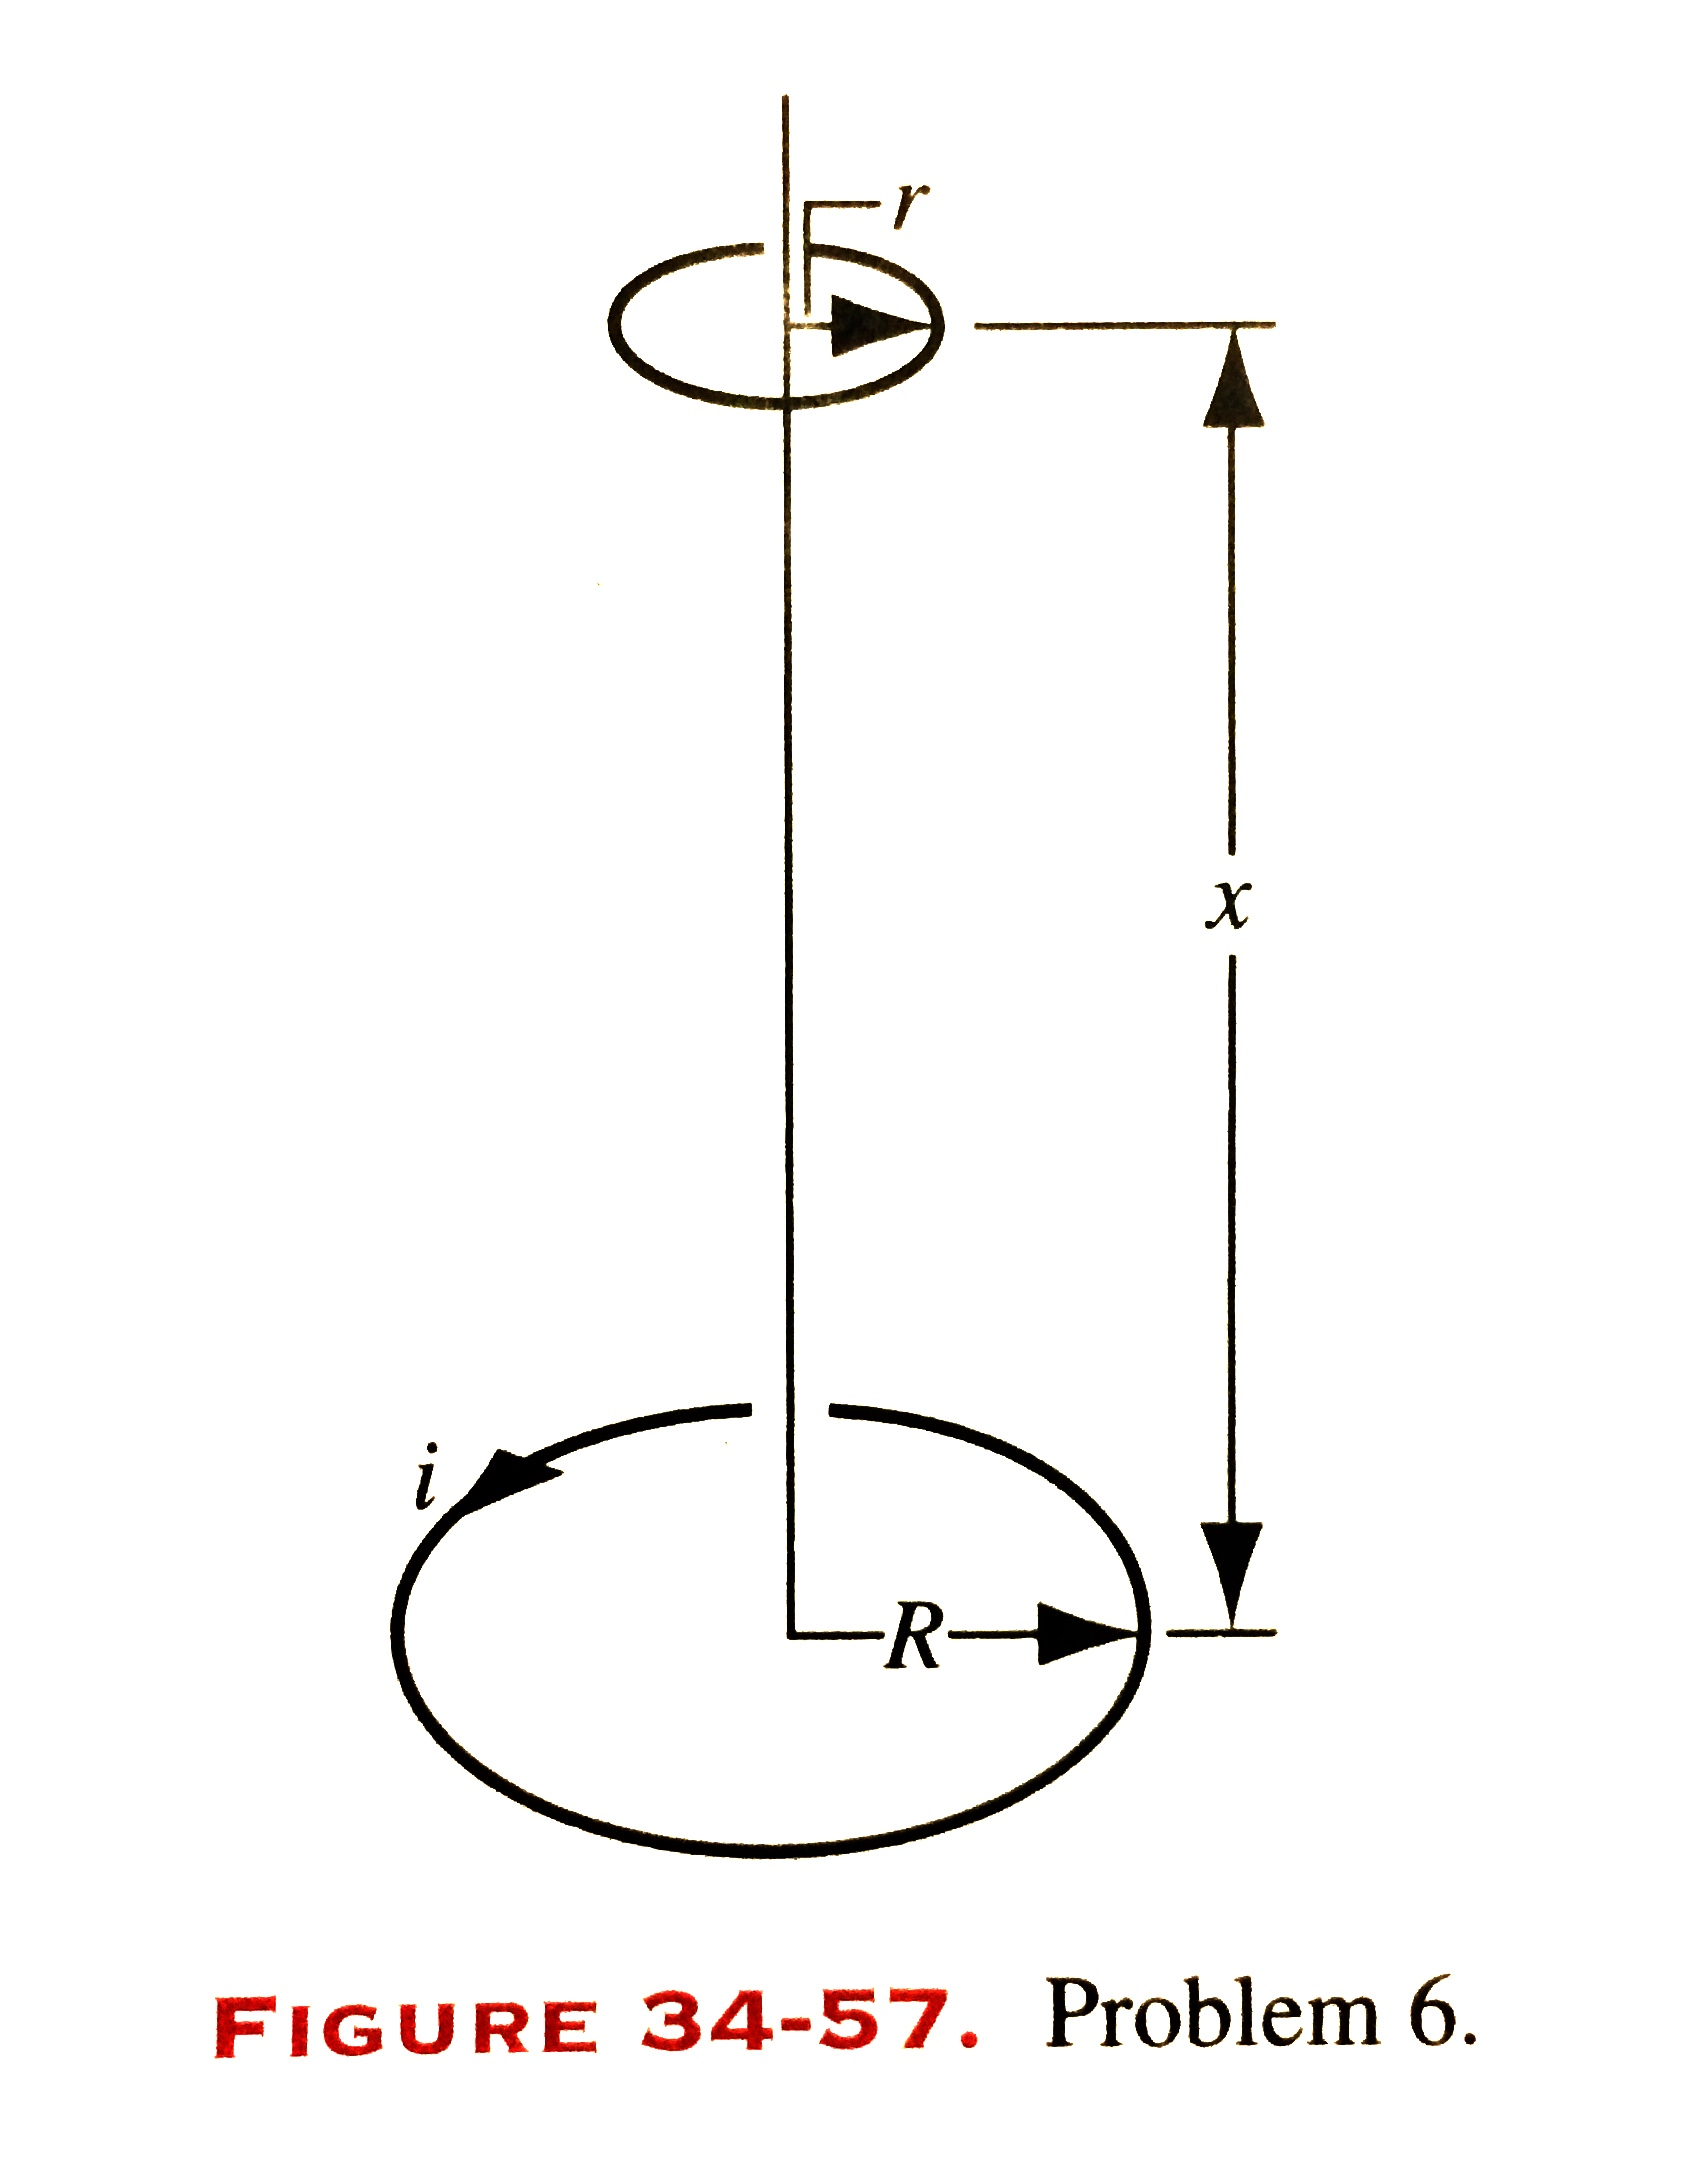
\includegraphics[scale=0.1]{02.jpg}
\end{center}
\end{problem}
\begin{solution}
\end{solution}
\newpage


\end{document}